\documentclass{jsarticle}
\usepackage[dvipdfmx]{graphicx}

\title{楽しい運動計測実習に関するレポート}
\date{\today}
\author{奥屋 直己}

\usepackage[height=26cm,width=16cm]{geometry}

\graphicspath{{./images/}}

\begin{document}

\maketitle

\section{実験の目的}

今回別の実験で腕を90度に曲げた状態でおもりを持ち、そのときの上腕二頭筋と上腕三頭筋の筋電位を計測するという実験を行った。そのとき、上腕二頭筋はもちろん大きく反応したが、上腕三頭筋の筋電位も反応した。なぜ腕を伸ばすはずの筋肉が反応したのだろうか。今実験では腕を伸ばす、曲げるの繰り返し運動を行うこのにより、求めていく。

\section{手法}

\subsection{実験}

今実験は右腕を水平面内で伸ばす、曲げるの繰り返し運動を行い、手首、肘、肩の3点の軌道と筋電の波形を計測した。被験者には指示せずに動かしやすい速度で動かす場合と、それよりも速く動かす場合の2つを指示した。3点の軌道の計測は、それぞれに反射マーカーをつけ、真上に設置した高速度カメラを使った。筋電の計測は、上腕二頭筋と上腕三頭筋に筋電計用電極を取り付け計測した。
それぞれ、サンプリングは筋電が200 [Hz]、軌道を1000 [fps]とし、同時パルス発生装置を使い、開始時刻を同期した上で20秒間計測した。この実験では2人の被験者で行った。ただし、1人はデータがうまく取れなかったため、データは実質1人分となった。
\subsection{解析}

今回は筋電センサ(LOGICAL PRODUCT:ワイヤレス筋電センサ乾式)による筋電データとモーションキャプチャ(Library:Move-tr/3D)による運動軌道データを別々のプログラムで作成する。

\subsubsection{筋電データ}

筋電データには計測したデータの他にノイズが混ざっていると予測されるため、データの1~40Hzに対してバンドパスフィルタ(3次バターワークス)をかけることにより、低周波のノイズを除去した。また、単純にバンドパスフィルタをかけるとデータのピーク位置が実際のデータよりもすこしおそくなってしまう。そのためpythonのfiltfilt関数を使うことにより、順方向と逆方向の両方から1回ずつフィルタをかけ、ズレをなくした。

次にC言語で筋肉の活動度(a(t))を以下の式で評価した。tは時間[s]×$10^3$で求まる。

\begin{equation}
a(t)=\frac{1}{\Delta{T}}\int^{t+\Delta{T}/2}_{t-\Delta{T}/2} |E(t)|dt
\end{equation}

E(t)は筋電位、幅$\Delta{T}$の窓を200 [frame]とした。サンプリングは1000 [fps]なので、$t\pm\Delta{T}/2$より、$\pm0.1$ [s]間での筋電位の上昇度を算出することができた。

\section{結果}

図\ref{fig:motion1}が指示していない速さでの腕の軌道、図\ref{fig:motion2}が速く動かす時の腕の軌道である。この2つの図を比較すると、図\ref{fig:motion2}が速さが速い分、線の密度とブレは大きくなるが、軌道に大きな差がない。このことから、速度による違いのみ抽出できる。図\ref{fig:EMG1}を見ると、上腕二頭筋の筋電位の山と、上腕三頭筋の筋電位の山がほぼ同じ所で発生していることがわかる。しかし、図\ref{fig:EMG2}を見ると少しわかりづらいが、上腕二頭筋の筋電位が山のとき、上腕三頭筋は谷になっており、指示していない速さの時と逆となった。また、指示していないときの上腕三頭筋の筋電位はおよそ0.005〜0.09 [mV]、速く動かしたときは、およそ0.06〜0.14 [mV]となった。さらに上腕三頭筋ではそれぞれ、0.01〜0.03 [mV]と0.04〜0.09 [mV]となり、上腕二頭筋と上腕三頭筋の筋電位の最小値と最大値は両方共とも速く動かした方が大きくなっている。

\begin{figure}[h]
  \begin{center}
    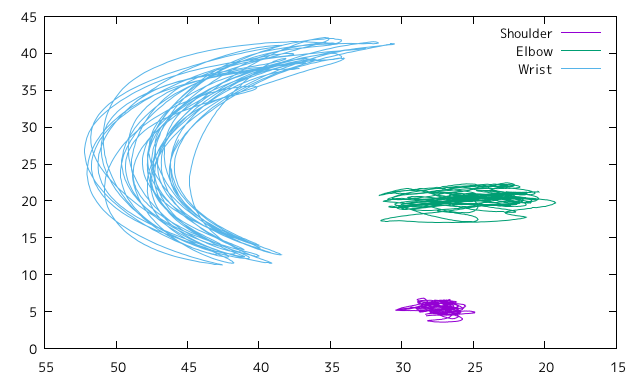
\includegraphics[clip,width=150mm]{Graph_2.png}
    \caption{指示していない速さでの運動での手首、肘、肩の3点の軌道(青=手首の軌道,緑=肘の軌道,紫=肩の軌道)。肘と肩はほぼ一定の位置で手首の軌道のみ大きく動いており、指示通りに腕を動かせていることがわかる。\label{fig:motion1}}
  \end{center}
\end{figure}

\begin{figure}[h]
  \begin{center}
    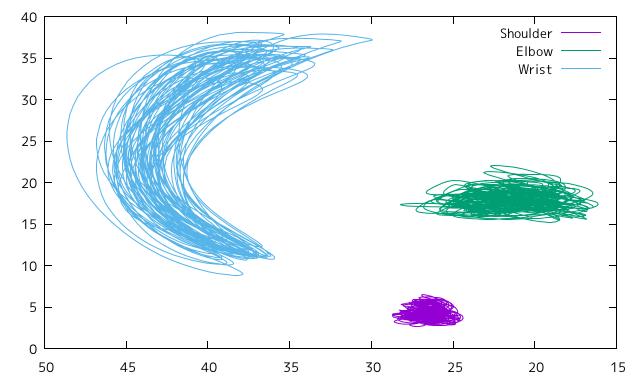
\includegraphics[clip,width=150mm]{Graph_3.png}
    \caption{図\ref{fig:motion1}よりも速く動かすように指示した場合の手首、肘、肩の3点の軌道(青=手首の軌道,緑=肘の軌道,紫=肩の軌道)。 図\ref{fig:motion1}と同様に手首のみが大きく動いており、指示通りに動かせていることがわかる。\label{fig:motion2}}
  \end{center}
\end{figure}

\begin{figure}[h]
  \begin{center}
    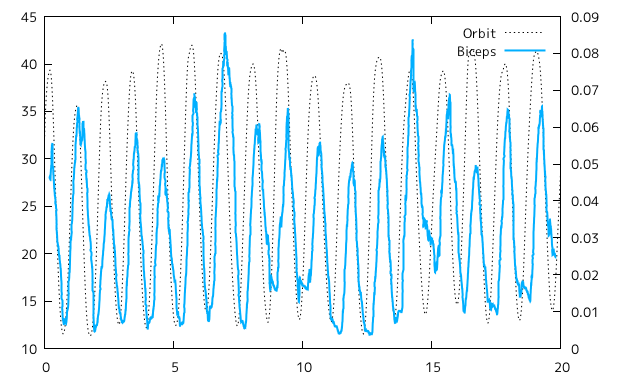
\includegraphics[clip,width=120mm]{Graph_4.png}
    \caption{指示していない速さで運動した時の上腕二頭筋と上腕三頭筋の筋電位(上腕二頭筋=青,上腕三頭筋=緑)。どちらの筋電にも腕の運動に合わせて振動している。 \label{fig:EMG1}}
  \end{center}
\end{figure}

\begin{figure}[h]
  \begin{center}
    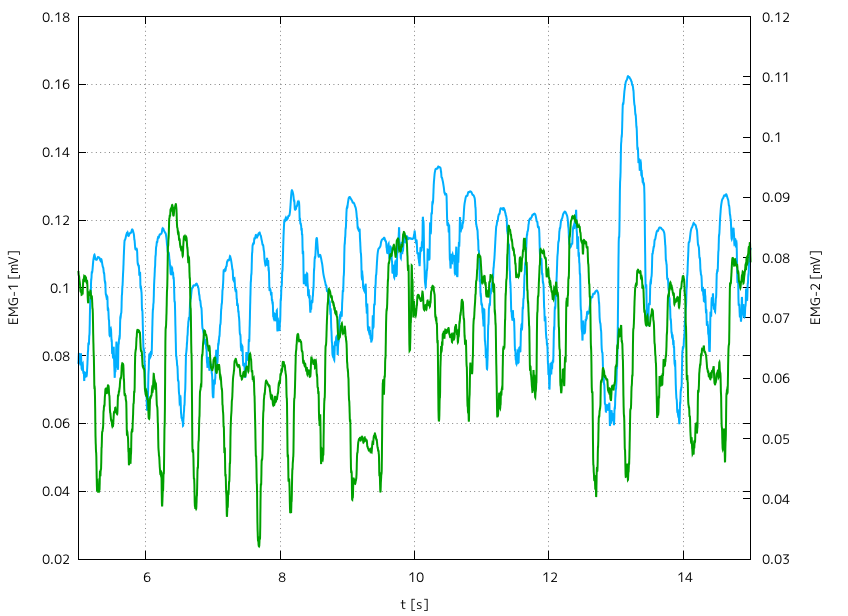
\includegraphics[clip,width=120mm]{Graph_5.png}
    \caption{速く動かす運動をした時の上腕二頭筋と上腕三頭筋の筋電位(上腕二頭筋=青,上腕三頭筋=緑)。左側のY軸が上腕二頭筋、右側のY軸が上腕三頭筋の筋電位を表す。 どちらの筋電にも腕の運動に合わせて振動している。\label{fig:EMG2}}
  \end{center}  
\end{figure}

\section{考察}
結果から指示していない速さのとき、上腕二頭筋と上腕三頭筋の筋電位の山がほぼ同じところで発生している。このことより、ゆっくり腕を曲げようとするとき、無意識にブレーキをかけながら動かすくことにより、一定の速度で動かそうとしているのではないかと考える。証拠に図\ref{fig:EMG1}をみると、上腕二頭筋が小さくなるに連れて少し遅れて上腕三頭筋も小さくなっている。逆に速く動かすときはブレーキをかける必要性はなくなるため、上腕二頭筋の筋電位が山のとき、上腕三頭筋の筋電位は谷となると考える。これらのことから、腕を90度に曲げた状態でおもりを持ち、これを保とうとするとき、上腕二頭筋だけだと、上方向に大きく動きすぎてしまうのではないかと考える。これに対してブレーキをかけることにより、90度を保とうとするのではないかと考える。
\end{document}